\section{Region Identification}

Visual breakdowns of the types of regions identified and their counts
for each \textit{Trichoderma} assembly are shown in figure
\ref{fig:regions-sankey}. We will first discuss the types of regions,
beginning with fully support regions. These regions labelled `Full
Support', are sections of genomic sequence where each gene finder
agrees that a gene is present in some form. These fully supported
regions are then broken down into two categories, based on whether or
not the models from each gene finder agree on the start and stop
positions of the gene model. Regions that have support from more than
one gene finder, but not all, are labelled regions with `Partial
Support'. These regions are also broken down in to two sub-regions
based on whether or not the gene predictions agree on the start and
stop positions of the gene. Regions with support from only one gene
finder are labelled as singletons.

\begin{figure}[h!]
  \centering
  \begin{subfigure}{0.9\textwidth}
    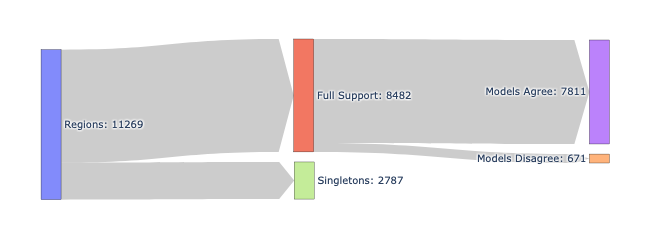
\includegraphics[width=\textwidth]{figures/dc1-region-breakdown.png}
    \label{fig:dc1-regions}
    \caption{DC1}
  \end{subfigure}
  \begin{subfigure}{0.9\textwidth}
    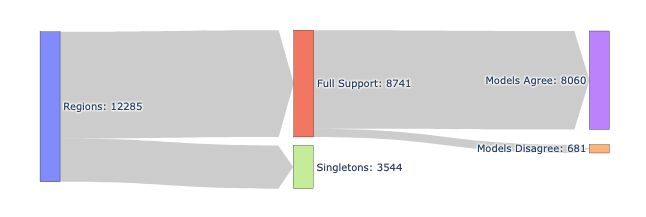
\includegraphics[width=\textwidth]{figures/tsth20-region-breakdown.png}
    \label{fig:tsth20-regions}
    \caption{Tsth20}
  \end{subfigure}
  \begin{subfigure}{0.9\textwidth}
    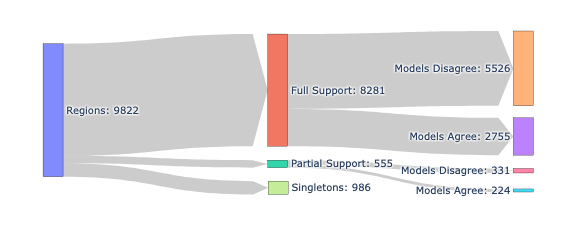
\includegraphics[width=\textwidth]{figures/t-reesei-region-breakdown.png}
    \label{fig:t-reesei-regions}
    \caption{\textit{T. reesei}}
  \end{subfigure}
\end{figure}
\begin{figure}[h!]
  \ContinuedFloat
  \centering
  \begin{subfigure}{0.9\textwidth}
    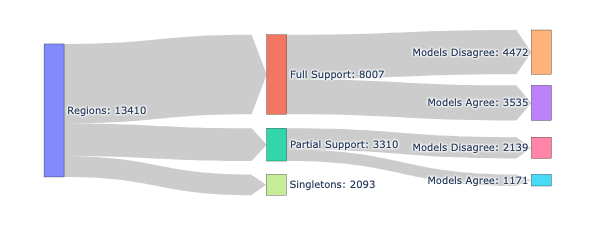
\includegraphics[width=\textwidth]{figures/t-harzianum-region-breakdown.png}
    \label{fig:t-harzianum-regions}
    \caption{\textit{T. harzianum}}
  \end{subfigure}
  \begin{subfigure}{0.9\textwidth}
    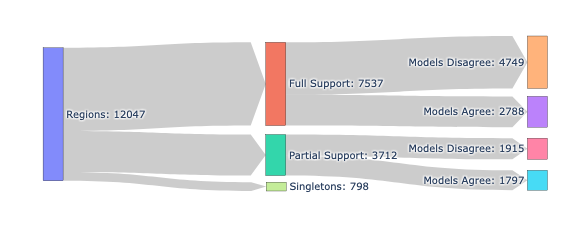
\includegraphics[width=\textwidth]{figures/t-virens-region-breakdown.png}
    \label{fig:t-virens-regions}
    \caption{\textit{T. virens}}
  \end{subfigure}
  \caption[Breakdown of identified regions]{Figures showing breakdowns
    of genomic regions identified by the region finding
    process. Regions with supporting predictions from all gene finders
    included in this analysis are labelled with `Full Support'. Fully
    supported regions are then broken down into regions where gene
    models agree on the start and stop positions of the genes, and
    those that do not. Regions labelled with `Partial Support' are
    regions with supporting gene predictions from more than one gene
    finder, but not all. Partially supported regions are also broken
    down into regions in which gene finders agree on the start and
    stop positions of the gene, and those that do not agree. Regions
    with gene predictions from only one gene finder are labelled as
    singletons.}
  \label{fig:regions-sankey}
\end{figure}

Looking at DC1 and Tsth20 in figure \ref{fig:regions-sankey}, it
appears that Braker2 and GeneMark predict genes in the same regions in
the majority of cases. For regions with full support, the models also
tend to agree on the start and stop positions of the gene in that
region. This is not generally the case as we will see
later. \textit{Trichoderma reesei} contains the fewest number of
regions, which seems to scale appropriately with the total number of
predicted genes. The vast majority of the regions are fully or
partially supported by Braker2, GeneMark and RefSeq, with only 10
percent of the regions being single predictions. The most interesting
thing here is the number of fully supported regions that disagree on
start and stop positions of the gene(s) in that region. There is
clearly a difference in the gene models being produced by these gene
finders. If there is disagreement on the start and stop positions of a
gene, then there is likely disagreement on the number and location of
exons and introns within the gene model as well. In the case of
partially supported regions, there is more disagreement than
agreement, but that may come as less of a surprise as there is already
disgreement on the presence of a gene at all. Gene finding behaviour
in regions from \textit{T.harzianum} and \textit{T. virens} differ
from the other assemblies in the split between fully and partially
supported regions. There seems to be fewer regions with full support
from all gene finders and the reason why is unclear. The gene models
in each region, whether fully or partially supported, still tend to
disagree on start and stop positions of the genes more often than
agree
